\documentclass[11pt, a4paper]{article}
\usepackage[a4paper, margin=1in]{geometry}

\usepackage{adjustbox}
\usepackage{mathtools}
\usepackage{amsmath}
\usepackage{amssymb}
\usepackage{amsthm}

\usepackage{pgfplots}
\usepackage{listings}
\usepackage{color}
\usepackage{tikz}

\usepackage{textcomp}
\usepackage{soul}

\usepackage[hidelinks]{hyperref}
\pgfplotsset{width=7.5cm,compat=1.12}
\usepgfplotslibrary{fillbetween}
\pgfplotsset{compat=1.8}
\usepgfplotslibrary{statistics}
\usepackage[makeroom]{cancel}
\title{\bf{Homework \textnumero 10}}
\author{Author: David Oniani
\\
\ \ \ Instructor: Dr. Eric Westlund}
\date{March 13, 2019}

\usepackage{listings}
\usepackage{color}

%%%%%%%%%%%%%%% S E T S %%%%%%%%%%%%%%%
\newcommand{\nats}{\mathbb{N}}
\newcommand{\ints}{\mathbb{Z}}
\newcommand{\rats}{\mathbb{Q}}
\newcommand{\reals}{\mathbb{R}}
\newcommand{\irrats}{\mathbb{I}}

\newcommand{\pnats}{\mathbb{N}^+}
\newcommand{\pints}{\mathbb{Z}^+}
\newcommand{\prats}{\mathbb{Q}^+}
\newcommand{\preals}{\mathbb{R}^+}
\newcommand{\nreals}{\mathbb{R}^-}

\newcommand{\nints}{\mathbb{Z}^-}
\newcommand{\nrats}{\mathbb{Q}^-}
%%%%%%%%%%%%%%%%%%%%%%%%%%%%%%%%%%%%%%%

% Calligraphy
\newcommand\und[1]{\underline{\smash{#1}}}

% Operators
\DeclarePairedDelimiter\abs{\lvert}{\rvert}
\DeclarePairedDelimiter\ceil{\lceil}{\rceil}
\DeclarePairedDelimiter\floor{\lfloor}{\rfloor}

% Other
\newcommand{\rarr}{\rightarrow}

\definecolor{dkgreen}{rgb}{0,0.6,0}
\definecolor{gray}{rgb}{0.5,0.5,0.5}
\definecolor{mauve}{rgb}{0.58,0,0.82}
\definecolor{backcolour}{rgb}{0.95,0.95,0.92}

\lstset{
backgroundcolor=\color{backcolour},
aboveskip=3mm,
belowskip=3mm,
showstringspaces=false,
columns=flexible,
basicstyle={\small\ttfamily},
numbers=left,
numberstyle=\normalsize\color{gray},
keywordstyle=\color{blue},
commentstyle=\color{dkgreen},
stringstyle=\color{mauve},
breaklines=true,
breakatwhitespace=true,
tabsize=4
}


\begin{document}
\maketitle
\begin{itemize}
\item[15.2]
As boldface number 39\% is out of all Democrat voters, it is the parameter.\\
As boldface number 35\% is out of all Republican voters, it is the parameter.\\
As boldface number 33\% is out of the \und{sample} of 250 subjects, it is the statistic.

\item[]
\item[]

\item[15.5]
Most of the time, loss from apartment damage is large and it is very probable
that company will lose a lot of money. On the other hand, if the number of policies
is very big (thousands of policies), then only a few of these thousands will suffer from
loss apartment damage and income from the rest of the policies will account for these financial
loses of the company. This the consequence of LLN (Law of Large Numbers).

\item[]
\item[]

\item[15.6]
\begin{itemize}
\item[(a)]
The population would be all of US adults.\\
The distribution describes the distribution of the number
of minutes of sleep per night an adult gets.\\
It is a normal distribution with the mean of 528.8
minutes and the standard deviation of 137.2 minutes.

\item[]

\item[(b)]
The sampling distribution of $\overline{x}$ describes
the distribution of the sample means of all possible
samples of size $n$.\\
It is a normal distribution with the mean of 528.8 minutes
and the standard deviation of 13.72 minutes.
\end{itemize}

\newpage

\item[15.7]
\begin{itemize}
\item[(a)]
Below is the histogram for this data.
\begin{center}
    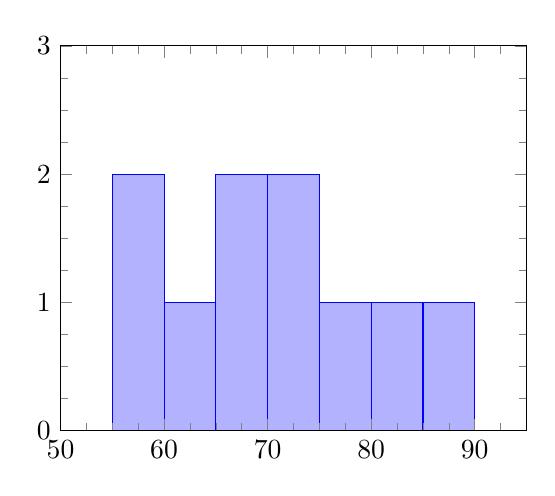
\begin{tikzpicture}
        \begin{axis}[
            ymin=0, ymax=3,
            xmin=50, xmax=95,
            minor y tick num = 3,
            minor x tick num = 3,
            area style,
            ]
        \addplot+[ybar interval, mark=no] plot coordinates { (55, 2) (60, 1) (65, 2) (70, 2) (75, 1) (80, 1) (85, 1) (90, 1)};
        \end{axis}
    \end{tikzpicture}
\end{center}

\item[]

\item[(b)]
$\mu = \dfrac{86 + 63 + 81 + 55 + 72 + 72 + 65 + 66 + 75 + 59}{10} = 69.4$.

\item[]

\item[(c)]
I shuffled the list of these values and took the first 4.
Below is the \texttt{Python} code.

\item[]
\item[]
\begin{verbatim}
from random import shuffle


def main():
    data = [86, 63, 81, 55, 72, 72, 65, 66, 75, 59]
    shuffle(data)
    print(data[:4])  # prints out [59, 75, 66, 81] on the first try


if __name__ == '__main__':
    main()
\end{verbatim}
\item[]
\item[]

Thus, using SRS, we got 4 datapoints 59, 75, 66, and 81.
Now, we can calculate the\\\\
sample mean, and finally get that $\overline{x} = \dfrac{59 + 75 + 66 + 81}{4} = 70.25$.

\item[]

\item[(d)]
Let's modify the code above to do the shuffling 10 times.

\item[]
\item[]
\begin{verbatim}
from random import shuffle
from statistics import mean
    
    
def main():
    data = [86, 63, 81, 55, 72, 72, 65, 66, 75, 59]
    avgs = []

    for i in range(10):
        shuffle(data)
        avgs.append(mean(data[:4]))

    print(avgs)


if __name__ == '__main__':
    main()
\end{verbatim}
\item[]
\item[]

On the first try, we got that 10 averages
are 73.5, 64, 68.25, 64.5, 65, 74.5, 63.75, 71, 73.25, and 65.
The values in the sorted order are 63.75, 64, 64.5, 65, 65, 68.25, 71, 73.25, 73.5, and 74.5.
Below is the histogram for the data.
\begin{center}
    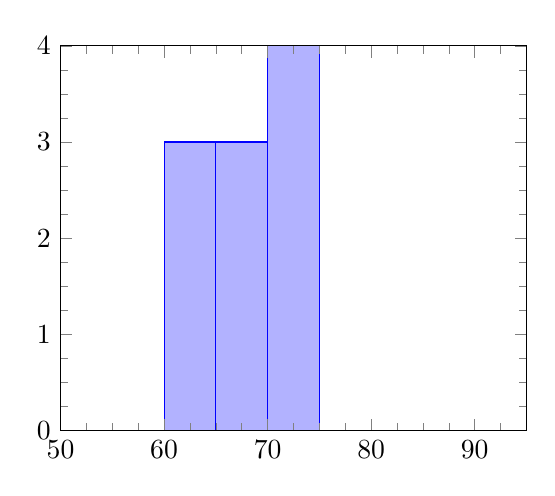
\begin{tikzpicture}
        \begin{axis}[
            ymin=0, ymax=4,
            xmin=50, xmax=95,
            minor y tick num = 3,
            minor x tick num = 3,
            area style,
            ]
        \addplot+[ybar interval, mark=no] plot coordinates { (60, 3) (65, 3) (70, 4) (75, 4)};
        \end{axis}
    \end{tikzpicture}
\end{center}

\item[]

The center of the histogram is really close to $\mu = 69.4$ as the centerpoint is $68.275$.
Compared to the distribution in the part (a) of the exercise, this distribution has smaller
spread. Besides, this distribution seems to be more ``normal'' than that of the part (a) of the
exercise.
\end{itemize}

\item[]
\item[]

\item[15.8]
\begin{itemize}
\item[(a)]
If we take a lot of samples, the average of the values of $\overline{x}$
from these samples will be very close to $\mu$. Therefore, the sampling
distribution of $\overline{x}$ has a center at the population mean $\mu$.

\item[]

\item[(b)]
Put is simply, if we have more information, we have better results.
In other words, larger sample yields more trustworthy results.
\end{itemize}

\item[]
\item[]

\item[15.9]
\begin{itemize}
\item[(a)]
The sampling distribution of $\overline{x}$ is $N(115, \frac{25}{\sqrt{100}} )$
which is the same as $N(115, 2.5)$\\
Using Table A, we get $P(112 < x < 118) = 0.8849 - 0.1151 = 0.7698$. Therefore, the
probability is 0.7698.

\item[]

\item[(b)]
The sampling distribution of $\overline{x}$ is $N(115, \frac{25}{\sqrt{1000}} )$
which is the same as $N(115, 0.7906)$\\
Using Table A, we get $P(-3.79 < x < 3.79) = 0.9998$. Therefore, the
probability is 0.9998.
\end{itemize}

\item[]
\item[]

\item[15.11]
Nope, unfortunately, it is not right.\\
The central limit theorem says that the histogram of \und{sample means}
will look more and more normal.\\\\
What student said is that the histogram of \und{sample values} will look more and
more normal. This is wrong as the histogram of sample values always looks like
the original population distribution. Therefore, if the population distribution
is not normal, it is most likely that the histogram of sample values is also not normal.

\item[]
\item[]

\item[15.13]
The state part is basically the description of the problem. It is already done.\\\\
\und{\textbf{PLAN}}\\\\
Since the sample size is large, according to the central limit theorem, the sampling
distribution of the sample mean is approximately normal. Our goal is to find a $z-score$
for the distribution. Once we know the $z$-score, we can use Table A to find the probability
and draw the conclusion.\\\\
\und{\textbf{SOLVE}}\\\\
$z = \dfrac{\overline{x} - \mu}{\sigma} = \dfrac{135 - 125}{\dfrac{300}{\sqrt{10000}}} \approx 3.33$.\\\\\\
Now, using Table A, we get that $P(\overline{x} \leq 135) = P (z < 3.33) = 0.9996$.\\\\
\und{\textbf{CONCLUDE}}\\\\
Since the probability of $P(\overline{x} \leq 135) = 0.9996$, it is almost $1$ (as $0.9996 \approx 1$)
and the company can safely assume that its average loss will be no greater that $\$135$.\\
Therefore, the answer is YES, company can safely base its rates on the assumption
that its average loss will be no greater that $\$135$.

\item[]
\item[]

\item[15.35]
The state part is basically the description of the problem. It is already done.\\\\
\und{\textbf{PLAN}}\\\\
We need to use the central limit theorem in order to approximate the probability.
We will also need to calculate $z$-scores (this is since we have to deal
with normal distributions; since the distribution of $x$ is normal, the sampling
distribution of the sample mean $\overline{x}$ is also approximately normal)\\\\\\\\
\und{\textbf{SOLVE}}\\\\
$z_1 = \dfrac{x - \mu}{\sigma} = \dfrac{10 - 13.3}{\dfrac{17}{\sqrt{40}}} \approx -1.23$\\
$z_2 = \dfrac{x - \mu}{\sigma} = \dfrac{5 - 13.3}{\dfrac{17}{\sqrt{40}}} \approx -3.09$\\\\\\
From Table A, we get that $P(\overline{x} > 10\%) = P(z > -1.23) = 0.8907$ and $P(\overline{x} < 5\%)
= P(z < -3.09) = 0.0010$.\\\\
\und{\textbf{CONCLUDE}}\\\\
There is approximately $89\%$ chance of getting average returns over $10\%$ and $0.1\%$ chance
of getting average returns less thatn $5\%$.

\item[]
\item[]

\item[15.36]
The state part is basically the description of the problem. It is already done.\\\\
\und{\textbf{PLAN}}\\\\
We will have to apply the central limit theorem as well as use Table A for calculating
$z$-scores. Since the distribution of $x$ is normal, the sampling distribution of the
sample mean $\overline{x}$ is also approximately normal. This is where $z$-scores will
come handy.\\\\
\und{\textbf{SOLVE}}\\\\
$z = \dfrac{x - \mu}{\sigma} = \dfrac{\dfrac{4000}{22} - 190}{\dfrac{35}{\sqrt{22}}} \approx 1.95$\\\\\\
From Table A, we get that $P(\text{TW} > 4500\%) = P(z > 1.95) = 0.0256$.\\\\
\und{\textbf{CONCLUDE}}\\\\
There is approximately $2.56\%$ chance that the total weight of passengers
exceeds 4500 pounds.

\item[]
\item[]

\item[15.38]
\begin{itemize}
\item[(a)]
Since the original distribution is normal, the sampling distribution of the sample mean is also
approximately normal. Now we can apply the $68-95-99.5$ rule.
According to the $68-95-99.5$ rule, 99.7\% of data (in the normal distribution)
lies within 3 standard deviations from the mean. Therefore, we get that $3\sigma = 1$
and $\sigma \approx 0.33$.

\item[]

\item[(b)]
We have to solve the equation $\dfrac{1}{3} = \dfrac{6.5}{\sqrt{n}}$.\\
We have:
\begin{align}
&\dfrac{1}{3} = \dfrac{6.5}{\sqrt{n}}\\
&\sqrt{n} = 19.5\\
&n = 380.25
\end{align}
Now, since the sample size is an integer, we have to round 380.25 up
and get that the sample size needs to be 381. Finally, we need SRS with
the size of 381 in order to reduce the standard deviation of $\overline{x}$
to the value found in part (a) of the exercise which is $\dfrac{1}{3}$.
\end{itemize}

\end{itemize}
\end{document}
